%\documentclass{acm_proc_article-sp}
\documentclass{sig-alternate}
\usepackage{amsmath}
\usepackage{amssymb}
\usepackage{listings}
\usepackage{courier}
\usepackage{multirow}

% Include PDF graphics, configure our images directory, and specify image types.
\usepackage{graphicx}
\usepackage{epsfig}
\graphicspath{{./images/}}
\DeclareGraphicsExtensions{.pdf,.jpeg,.png,.jpg}

% Style listings
\lstset{%rulesepcolor=\color{Gray},
        frame=single,                        	% Shadow box frame around code
        basicstyle=\scriptsize\ttfamily,        % Use small true type font
        showstringspaces=false,                 % Don't put marks in string spaces
        morecomment=[l][\color{Blue}]{...},     % Line continuation (...) like blue comment
}

\begin{document}

\title{Dynamic, Secure Resource Control in the Cloud}

\numberofauthors{1}

\author{
\alignauthor
Viswanath Nandina, Edward J. Nava, Jos\'e Marcio Luna, Christopher C. Lamb, Gregory L. Heileman, Chaouki T. Abdallah\\
       \affaddr{University of New Mexico}\\
       \affaddr{Department of Electrical and Computer Engineering}\\
       \affaddr{Albuquerque, NM 87131-0001}\\
       \email{\{vishu, ejnava, marcio, cclamb, heileman, chaouki\}@ece.unm.edu}
}

\conferenceinfo{CCSW' 12,} {October 19, 2012, Raleigh, NC, USA.} 
\CopyrightYear{2012} 
\crdata{978-1-4503-1005-5/11/10} 
\clubpenalty=10000 
\widowpenalty = 10000

\maketitle

\begin{abstract}
In this paper we describe the development of a system that provides security and performance controls over content in a cloud environment.  Using artifacts that are classed at different sensitivity levels associated with service level agreements (SLAs) describing how and where they can be used. Using an approach grounded in control theory we are able to successfully provision resources in a hybrid cloud environment that have dynamic security attributes customized for content slated for processing.  These provisioned resources are created to match both performance characteristics and specific sensitivity restrictions specified within associated SLAs.
\end{abstract}

\category{D.2.11}{Software}{Software Architectures}[Domain-specific Architectures]
\terms{Design, Performance, Security}
\keywords{Access Control, Interoperability, DRM, Usage Management}

\section{Introduction}\label{sec:introduction}
With the advent and widespread use of cloud computing, those responsible for a given usage managed resource are almost never those responsible for the computing systems, except at edge devices like mobile phones or other small profile computing devices.  Resources are regularly moved across national boundaries and regional areas without either the content owner's or creator's knowledge.  Furthermore, this kind of transfer is generally according to pre-established algorithms or data routing protocols over which users have no control.  Managing these issues requires new usage management capabilities that can run on platforms ranging from small, hand-held devices to nodes in large data centers.

Herein, we define usage management as the ability to control actions over resources and data across and within computing environments.  More than access control or digital rights management, usage management addresses with fine-grained control of all aspects of how a given digital resource is used.  As digital environments become more open over time, the need for usage management for resources that span utility computational environments (e.g. cloud provider systems) will become increasingly important \cite{ctrl:lamb-MCCCS,ctrl:lamb-SOSE}.

One of the central problems with respect to usage management application in cloud environments is the ability to specify and enforce specific levels of usage management over resources.  The essential mobility of information within private, public, and hybrid cloud environments makes this management virtually impossible currently, leaving system developers left with the sole option of designing proprietary information management capabilities.  These capabilities become more and more expensive to develop as computational environments become increasingly distributed, and are generally a nightmare to manage, both due to the proliferation of disparate technology throughout the available public and private cloudosphere. 

This work focuses on developing integrated SLAs that address both traditional performance measures as well as security and usage management directives.  We feel that cloud monitoring capabilities have over the past year reached the point at which commercial providers supply enough performance monitoring and system management primitives to begin to implement cloud-scale automatic management systems addressing data processing suitability from both performance and security perspectives.  For example, Amazon now supplies information through their CloudWatch product and provides a robust control interface via their Elastic Compute Cloud (EC2).  Likewise, private cloud infrastructure-as-a-service (Iaas) offerings like OpenStack and Eucalyptus provide similar control interfaces, simplifying control of hybrid systems.

%Herein, we develop the mechanisms to enable control based on SLA established performance and security measures.  We introduce a prototypical system architecture, security parameters, and control profiles based on widely used open-source tooling to establish a simple proof of concept.

\section{Contributing Work}\label{sec:motivation}
Over the past few years multiple service-based paradigms such as web services, cluster computing and grid computing have contributed to the development of what we now call cloud computing \cite{Bu:09}. Cloud computing distinctly differentiates itself from other service-based computing paradigms via a collective set of distinguishing characteristics:  market orientation, virtualization, dynamic provisioning of resources, and service composition via multiple service providers \cite{BuYeVeBrBr:09}. This implies that in cloud computing, a cloud-service consumer's data and applications reside inside that cloud provider's infrastructure for a finite amount of time.  Partitions of this data can in fact be handled by multiple cloud services, and these partitions may be stored, processed and routed through geographically distributed cloud infrastructures. These activities occur within a cloud, giving the cloud consumer an impression of a single virtual system.  These operational characteristics of cloud computing can raise concerns regarding the manner in which cloud consumer's data and applications are managed within a given cloud. Unlike other computing paradigms with a specific computing task focus, cloud systems enable cloud consumers to host entire applications on the cloud (i.e. software as a service) or to compose services from different providers to build a single system. As consumers aggressively start exploiting these advantages to transition IT services to external utility computing systems, the manner in which data and applications are handled within those systems by various cloud services will become a matter of serious concern \cite{Jamkhedkar:2010:IUM:1866870.1866885}.

A growing body of research has begun to appear over the past two years applying control theory to tuning computer systems.  These range from controlling network infrastructure \cite{ctrl:ariba-GL:2009} to controlling virtualized infrastructure and specific computer systems \cite{ctrl:wang-cgswrzh:2009}, \cite{ctrl:kjaer-kr:2009} to exploring feedforward solutions based on predictive modeling \cite{ctrl:abdelwahed-bsk:2009}.  Significant open questions remain within this field \cite{ctrl:Zhu:2009:CTB:1496909.1496922}, \cite{ctrl:hellerstein-sw:2009}.

\section{Conceptual Configuration}
Usage management incorporates specific characteristics of traditional access control and digital rights management incorporating encryption mechanisms, trust management, and trusted computing platforms \cite{Jamkhedkar:2010:IUM:1866870.1866885}.  In order to be effective, it must be flexible enough to provide users with opportunities for differentiation and extension, but interoperable enough to provide services across widely diverging computational environments.  In this paper, we use images as the controlled resources, where each image has a set of policies associated with it that describe the circumstances under which that image can be used.

Likewise, each user is associated with an identity that describes their credentials and environment information, also known as context. Usage management occurs when a user's identity information is compared with a resources' policies to determine if that user is qualified to use that particular resource.

Access control is utility to manage controlled access resources.  The various components of our access control model are:
\begin{itemize}

\item \textbf{Roles}: The roles table is used to record user's roles. There is an entry for each user. It consists of an id, which is a unique identifier that defines different type of roles, and another field called parent, which can be used to define inheritance.

\item \textbf{Resources}: The resource table is used to identify each resource whose access is being controlled. Each entry consists of an id, which is a unique identifier, and another field for the resource descriptor. A resource can be anything from a file to a service.

\item \textbf{RolesResources}: The RolesResouces is the access control mapping between the roles and resources. It consists of 3 fields. The first entry in the column identifies the user by Roleid. The second entry contains the id of a resource to which a user is authorized access. The third field defines the user's privileges for that resource.

\end{itemize} 

Our primary goal is to develop and implement a secure, robust, and inter-operable role-based usage management system for data transactions in cloud computing. This system will merge traditional usage management systems with modern cloud computing technologies~\cite{Jamkhedkar:2010:IUM:1866870.1866885}.

The usage management system envisioned consists of an ACL containing a usage hierarchy where every person must adopt one or more of two explicit roles: admin or user. An admin sits atop the hierarchy and therefore has the most privileged access to resources. A user, generally, has limited access only to those resources approved by the usage management policy for that user. Similar to the hierarchal structure of an object-oriented programming language, every admin is a user, but every user is not an admin. Based on an individual's role they are assigned an identification number specific to the role. If someone requires multiple roles then unique identifications must be created for each of those roles. This system access policy is called Role-Based Access Control (RBAC). 

Every user and admin has access to certain resources defined by the user and admin's context of access control.  To formalize the confidentiality, integrity, and authenticity of data resources we have defined the context of access control by the tuple S = \{C, I, A\}, where C is a bit indicating the confidentiality of the data resource, I is a bit indicating the integrity of the data resource, and A is a bit indicating the authenticity of the data resource. That is, each bit defines the high or low status of confidentiality, integrity, and authenticity and is syntactically represented by the letters H or L.  Hence, there are 8 possible list orderings of access control.  These orderings indicate the degree of access admin's and user's have within the system. Therefore, if a user wishes to access a resource with some or all of the 8 possible degrees of security, the user must have the appropriate authoritative credentials and clearance rights.  These usage policy management rights are determined by the private party and then strictly controlled in the system's infrastructure to ensure the party complete security and control over whom is able to view specific data resources.

Each user's access to any data resources is controlled through a database. The database is designed to control access by assigning a unique identification number to each role, that is, a number corresponding to each role, not each user. Based on the credentials of the user, the user is presented a list of resources the user is allowed to access and is informed there exists a private encryption key for each resource. If the user sufficiently meets the qualifications for viewing the data resource, our custom Cloud Manager software provisions the data based on the degree of security particular to the data. The Cloud Manager instantiates the Virtual Machine using the corresponding private key to the specific Virtual Machine. Since there are 8 degrees of security as defined by the ordered tuple attributes, our software selects one of 8 image instances and allows the data to be accessed through one of 8 Virtual Machines.  Each image instance and Virtual Machine only handles data with the appropriate degree of security it is specified to manage. When a user decides to launch an image, the Cloud Manager will query a resource table for the three attributes of the image intended to facilitate that resource. For example, if all the three security attributes of the image are SC \{H,H,H\}, then the image can be executed in a Virtual Machine that also has all of these attributes set to SC \{H,H,H\}. 

Resources are typically stored in a cloud computing repository such as Amazon Simple Storage service (Amazon S3). Amazon S3 can be used to store and retrieve data in a very flexible manner via the web. It provides redundant storage and the management is transparent to the user.

\subsubsection{System Architecture/Model}
\begin{figure}[h]
  \begin{center}
    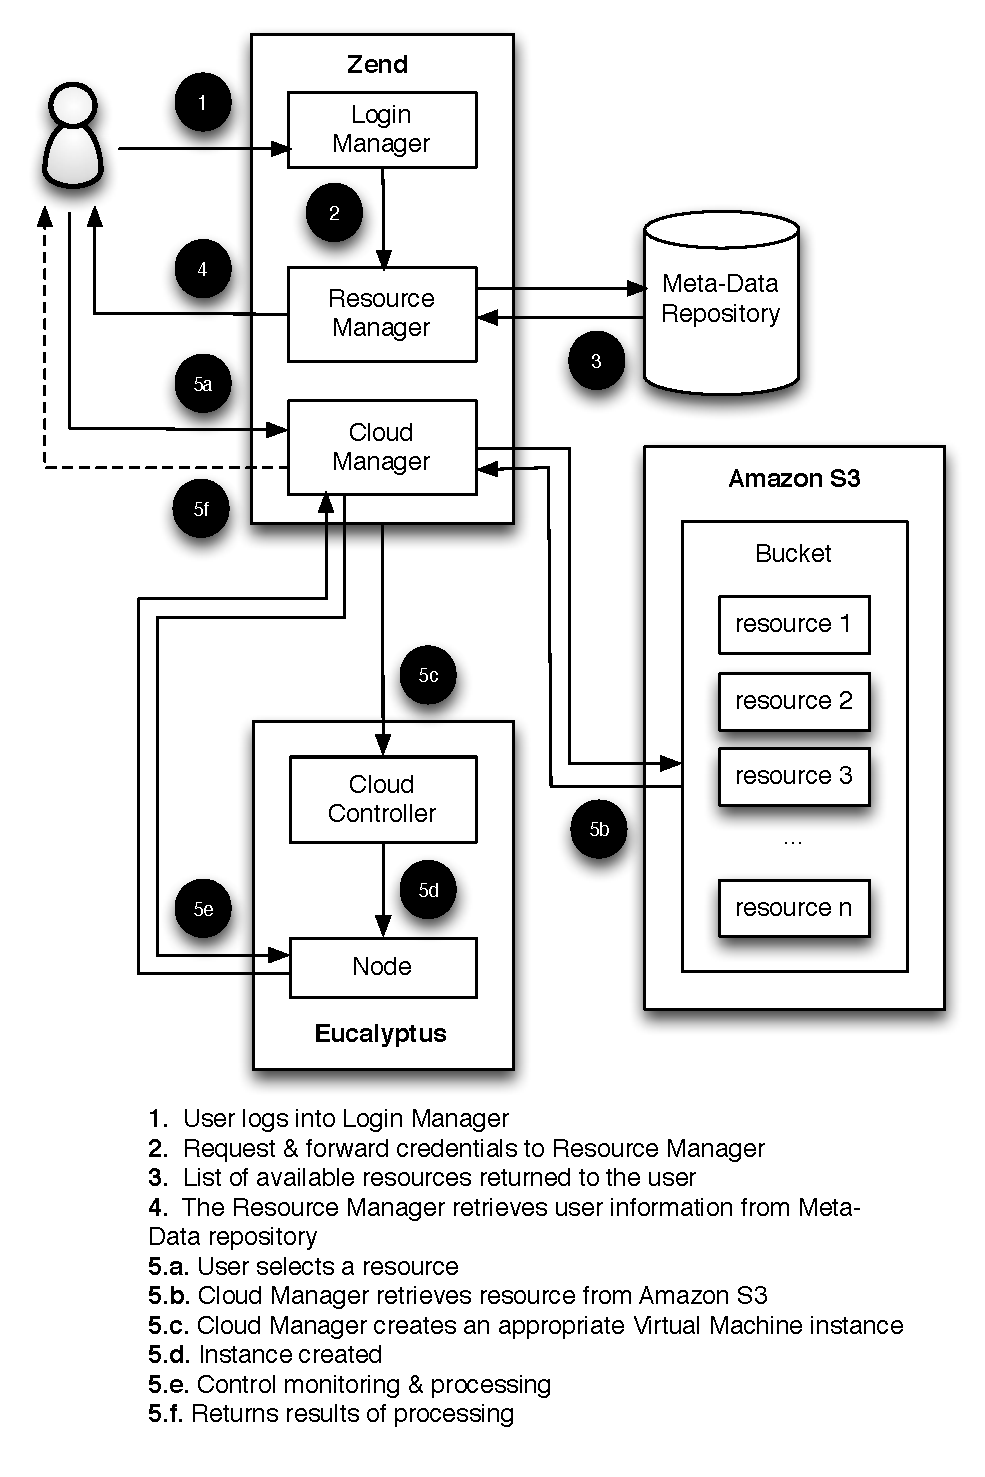
\includegraphics[width=.49\textwidth]{component}
  \end{center}
  \caption{Component Diagram of Usage Management for a Cloud-Based System}
  \label{fig:convergence}
\end{figure}


%1.  User logs into Login Manager\\
%2.  Request \& forward credentials to Resource Manager\\
%3.  List of available resources returned to the user\\
%4.  The Resource Manager retrieves user information from Meta-Data repository\\
%5.a. User selects a resource\\
%5.b. Cloud Manager retrieves resource from Amazon S3\\
%5.c. Cloud Manager creates an appropriate Virtual Machine instance\\
%5.d. Instance created\\
%5.e. Control monitoring \& processing\\
%5.f. Returns results of processing

The operational details of our usage management system are visualized in Figure 1.  By means of a web browser user interface, the user is presented with a login dialog box. The user enters user credentials to log into the system. The credentials are forwarded to the Resource Manager. The Resource Manager queries a Meta-Data repository to get information about the user.  Once the user's identification has been authenticated, a list of available resources is presented on the user's browser.  This list of resources varies depending on user context. If the user selects a resource, the Cloud Manager software retrieves the desired resource from a cloud computing repository like Amazon S3.  The Cloud Manager software then instantiates an appropriate Virtual Machine specified to handle resources with the same security context. The Cloud Manager also monitors the instance and returns references about the performance of the node to the Cloud Manager.  Using the our control-theoretic approach, we regulate the performance measures of the system that are covered by SLA requirements.

\subsubsection{Implementation}
\begin{figure}[h]
  \begin{center}
    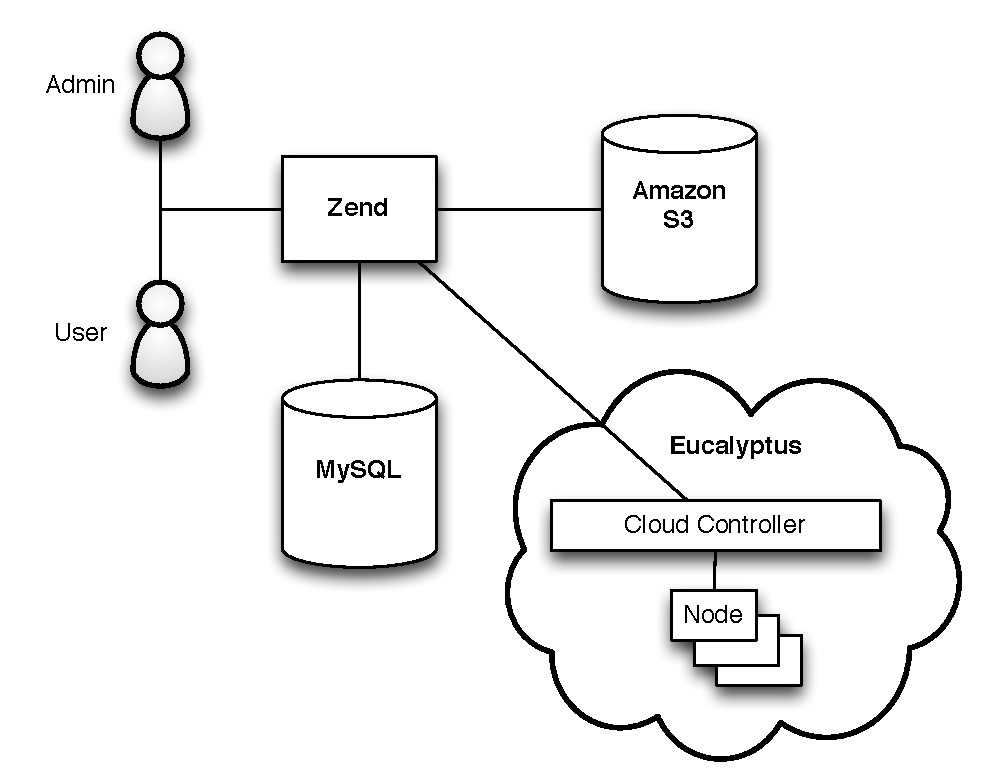
\includegraphics[width=.49\textwidth]{Technology_Architecture}
  \end{center}
  \caption{Technology Architecture}
  \label{fig:convergence}
\end{figure}

The implementation of the system is shown in Figure 2.  The application is written using Zend framework and we use MySQL for the database services. When a user logs in, we use Zend to authenticate and determine the role of the user. Once a user is authenticated we use ACL to decide what resources the user can access. Based on the resources available to the user we present the user with a list of images the user can run on a Virtual Machine. It is important to note the actual resources are stored in Amazon S3 and some of the features of the Eucalyptus cloud system have been omitted from our diagram for the sake of brevity.  If the user selects a resource, we query the resource table to get the appropriate keys and then execute the image in the virtual machine specified to manage resources with the appropriate security categories.  With the help of our software we monitor the VMs for performance as defined in the SLA requirements and control the VM appropriately.

\section{Systems and Control Approach}
In a cloud computing environment each application may have different performance measures, such as, response time, 
throughput or even number of instructions per second in the case of compute applications. Furthermore, since our main goal is
to control more than one performance measure by controlling one or more inputs of the system,
we consider the cloud model to be a Multiple-Input-Multiple-Output (MIMO) system.

The control method we use in our approach rely upon the availability of a mathematical model relating virtual resources
and performance measures of the system. Based on \cite{Nathuji-2010}, given an input vector 
$\mathbf{u}(n) = (u_{1}(n),\ldots,u_{q}(n))^{T}$ and a
state vector $\mathbf{y}(n) = (y_{1}(n),\ldots,y_{p}(n))^{T}$ of the cloud, the general MIMO
model of the cloud interactions is given by a set of nonlinear difference equations. The existent identification 
techniques for nonlinear systems are not suitable to be implemented in real-time, furthermore the amount of required
learning data for the identification algorithm turns out to be impractical except for the simple cases.

In previous works on data centers and cloud computing such as, \cite{Nathuji-2010},\cite{Yao-ACC-2010} and \cite{Luna-2011b}
a linear time-invariant realization of the system is accurate enough as long as the control inputs of the system are
constrained to a relatively "small`` interval. In the following section we provide a detailed description of the system
and a first candidate for the controller.

\begin{figure}[h]
  \begin{center}
    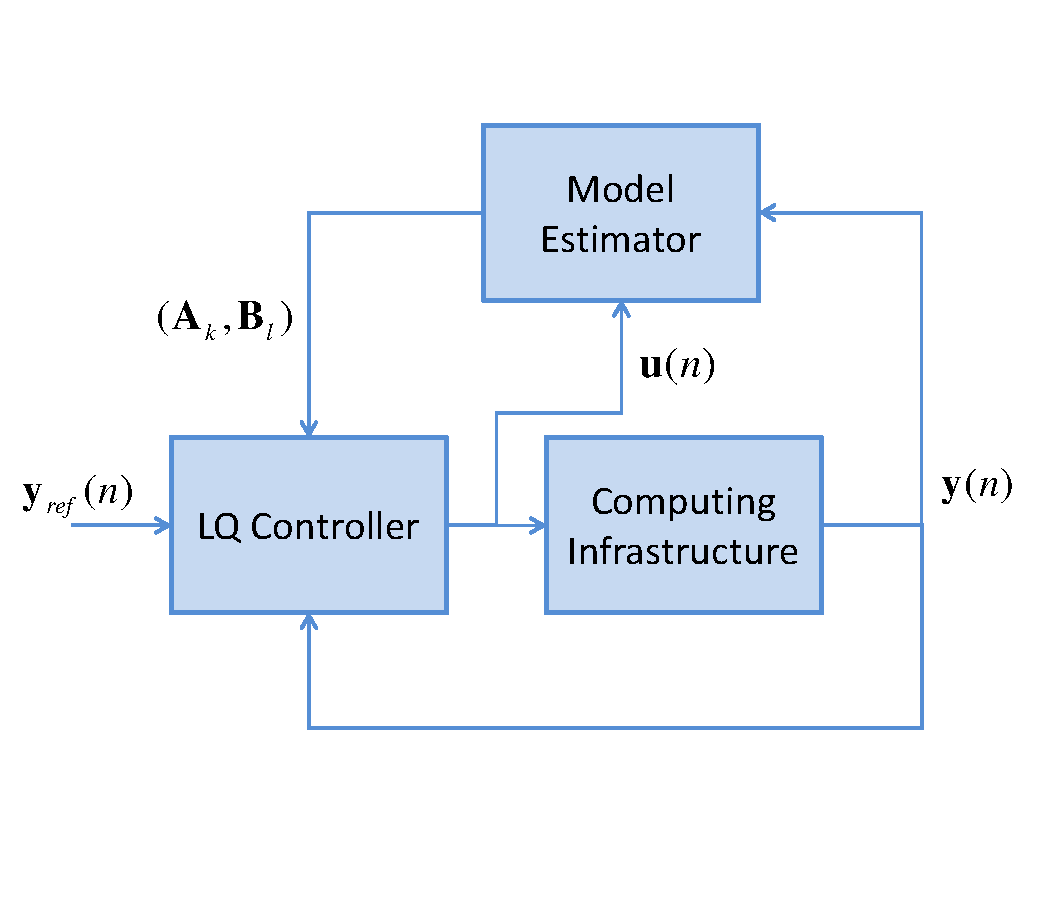
\includegraphics[width=.49\textwidth]{Fig_Closed_Loop}
  \end{center}
  \caption{Control Block Diagram}
  \label{fig:control}
\end{figure}

\subsection{Dynamic Model}
Our model is approximated by the following difference equations,
\begin{equation}
 \mathbf{y}(n) = \sum_{k=1}^{N}A_{k}\mathbf{y}(n-k)+ \sum_{l=0}^{M-1}B_{l}\mathbf{u}(n-l) + \mathbf{w}(n),
 \label{model}
\end{equation}
where $\mathbf{y} \in \Re^{p}$ is the state vector, $\mathbf{u} \in \Re^{q}$ is the input vector, 
$\mathbf{w} \in \Re^{q}$ is a zero-mean white-noise vector, 
and the system matrices $A_{k} \in \Re^{p \times p}$ and $B_{l} \in \Re^{p \times q}$ 
are to be estimated.

Now, by defining the matrix $X$ and the vector $\phi$ as follows,
\begin{equation}
 X = \left( B_{0},B_{1},\ldots,B_{M-1},A_{1},A_{2},\ldots A_{N} \right),
 \label{system}
\end{equation}
\begin{displaymath}
 \mathbf{\phi}(n) = ( \mathbf{u}(n)^{T},\ldots,\mathbf{u}(n-M+1)^{T},\mathbf{y}(n-1)^{T},\dots,\mathbf{y}(n-N)^{T})^{T},
\end{displaymath}
then we can reformulate the difference equation (\ref{model}) as,
\begin{displaymath}
\mathbf{y}(n) = X\mathbf{\phi}(n) + \mathbf{w}(n).
\end{displaymath}
Therefore, by getting an estimate $\hat{X}$ of the matrix $X$ we get a linear realization of the model based on the inputs
and outputs of the system.

The following iterative equations, based on \cite{Kulhavy-1987}, conform our Recursive Least Square (RLS)
estimator,
\begin{eqnarray}
 \mathbf{\varepsilon}(n+1) & = & \mathbf{u}(n+1) - \hat{X}(n)\mathbf{\phi}(n), \nonumber \\
\hat{X}(n+1) & = & \hat{X}(n)+\frac{\mathbf{\varepsilon}(n+1)(\mathbf{\phi})^{T}(n)P(n-1)}{\lambda + (\mathbf{\phi})^{T}(n)P(n-1)\mathbf{\phi}(n)}, \nonumber \\
P^{-1}(n) & = & P^{-1}(n-1) + \phi(n)(\phi)^{T}(n) \nonumber \\
& & + (\lambda - 1) \frac{(\mathbf{\phi})^{T}P(n-1)\mathbf{\phi}(n)}{[(\mathbf{\phi})^{T}(n)\mathbf{\phi}(n)]^{2}} \mathbf{\phi}(n)(\mathbf{\phi})^{T}(n) \nonumber.
\end{eqnarray}
where $P$ is the covariance matrix, $\lambda \in (0,1)$ is the forgetting factor and $\hat{X}$ is the estimate of $X$.
Notice from (\ref{system}) that the estimate $\hat{X}$ contains the desired estimate of the parameters of the systems.

\subsection{Linear Quadratic Control}
With the estimate of the MIMO system of the cloud, we proceed to design a Linear Quadratic control that minimizes the 
following cost function,
\begin{equation}
 J = (\mathbf{y}(k)-\mathbf{y}_{ref}(k))^{T}Q(\mathbf{y}(k)-\mathbf{y}_{ref}(k)) + u^{T}(k)Ru(k), \label{costf}
\end{equation}
where the matrix $Q \in \Re^{p \times p}$ is positive semi-definite and determines the level of accuracy of the regulated 
states, and $R \in \Re^{q \times q}$ is a positive definite matrix that penalizes the control effort \cite{Dorato-2000}.

By assuming no effect from the noise vector $\mathbf{w}$ we rewrite the system as,
\begin{displaymath}
 \mathbf{y}(n) = \mathbf{y}(n-1) + B_{0}u(n)
\end{displaymath}
then, from \cite{Liu-2007} we get the following control law that minimizes the cost function (\ref{costf}), while guaranteeing the stability
of the system,
\begin{eqnarray}
 &\mathbf{u}(n) = \left( (W\hat{B}_{0})^{T}W\hat{B}_{0}+Q^{T}Q \right)^{-1} \times& \nonumber \\ 
 &\left[ (W\hat{B}_{0})^{T}W \left(\mathbf{y}_{ref}(n+1) -\hat{X}(n)\tilde{\phi}(n) \right) + Q^{T}Q \mathbf{u}^{T}(n-1) \right].& \nonumber
\end{eqnarray}

Through this approach, we should be able to regulate the performance measures of the system that are covered by the
SLA and implemented through our policy based usage management of the cloud. One of the main concerns in this approach is the
implementation of our linear quadratic control to an IaaS environment. 
Specifically, in the EC2 service, the variations within Virtual Machines (VMs) instances
is limited to some discrete values, namely, small, large and extra-large intances. Therefore, the discrete-state and
discrete-time properties of the system imply some considerations when the SLA imposes references of the 
performance measures that are not reachable given the discrete-state constrain of the system. However, to overcome 
this particular issue, we restrict the regulation problem to satisfy only feasible values for all performance measures to
avoid oscillations or overshoots on the states.

\section{Security Category Analysis}
Our plan is to label resources (information) and systems using the NIST standards for security classification of Federal Information and Information Systems~\cite{FIPS199}.

The security objectives for both the information and the information systems are: confidentiality, integrity, and availability.  For both the information and the information systems, the impact of the compromise of each of these objectives is categorized as: low impact, moderate impact, or high impact.  A generalized format for expressing an information type security category as:
\newline
\newline
\begin{math}
SC= \{confidentiality,integrity,availability\}
\end{math}
\\

An overall system category is the high water mark value of the three individual objectives.  For example, a system with moderate impact for confidentiality and low impact for both integrity and availability is given an overall rating as a moderate impact system.

A security policy-based control system will contain a table with information system security category information that will be used as a basis for allowing or not allowing a operation on an individual cloud computing system.

\subsection{Protection Measures}
For each security category, we can use a number of mechanisms to achieve the necessary level of protection, integrity assurance, or availability.  The mechanisms that may be used for each level are proposed below.  For all transactions with data, we assume that a usage mechanism is available to control access as appropriate.  Once the user has been granted access to the data, the mechanisms below would be incorporated into an operating system image that will be loaded on newly instantiated VMs.

Additional protection can be achieved by using private or community cloud computing systems.  This approach would serve to eliminate the sharing of the base hardware with untrusted users, but also forces organizations to pay to install and maintain the systems.  This approach has its merits but also negates some of the cost savings than an organization could get by renting what they need, only when they need it.  As a result, we are focusing on measures that can be used in public cloud computing systems.  The specific measures we propose are shown below.

\begin{table}[ht]
\begin{tabular}{|c|p{2.5in}|}
\hline
Level &  Measures Or Mechanisms \\
\hline
H & Data encrypted while at rest, 
    Data transmitted in encrypted form (HTTPS, SSL, Tunnels) \\
\hline
M & Data transmitted in encrypted form (HTTPS, SSL, Tunnels) \\
\hline
L & Data handled and transmitted in the clear,
    Use standard OS file protection measures \\
\hline
\end{tabular}
\caption{Confidentiality}
\end{table}

\begin{table}[ht]
\begin{tabular}{|c|p{2.5in}|}
\hline
Level &  Measures Or Mechanisms \\
\hline
H & Data are signed with a secure hash [2],
    Data transmitted in encrypted form (HTTPS, SSL, Tunnels)\\
\hline
M & Data transmitted in encrypted form (HTTPS, SSL, Tunnels),
    Data are verified with a Message Authentication Code [3]\\
\hline
L & Data handled and transmitted in the clear,
    Use standard OS file protection measures, 
    Standard Parity checks used\\
\hline
\end{tabular}
\caption{Integrity}
\end{table}

\begin{table}[ht]
\begin{tabular}{|c|p{2.5in}|}
\hline
Level &  Measures Or Mechanisms \\
\hline
H & Data stored using Simple Storage System (S3),
    (Use built-in redundancy) \\
\hline  
M & Data stored using S3,
    (Use built-in redundancy)\\
\hline
L & Data are stored on local machines,
    Data stored using S3 \\
\hline
\end{tabular}  
\caption{Availability}
\end{table}

\subsection{Implementation}
VMs are instantiated to meet computational needs; the specific configuration of each can be controlled.  With no security controls, a user selects one from a set of images that can be used to launch the VM.  The image contains the operating system and other application software that is loaded into the VM when it is instantiated. 
 
Images can be configured with mechanisms to implement the functions required for each security category.  Images that process data with security triples of  SC\{H, *, *\}, SC\{M, *, *\}, SC\{*, H, *\}, and SC\{*, M, *\} should be configured to include intrusion detection system software, firewall software, virus checking software, and operations logging.  In addition, the operating systems should be configured to prevent the user from reconfiguring the operating system and application software.   (As good computer security practice, all images should include virus checking software.)

The security category triple yields a set of $3^{n}$ possible combinations.  With $n = 3$, this results in 27 different security categories to consider in a system design.  As a first step in simplifying the problem to make it more tractable, we will reduce each security objective to two values, low or high.  This reduces the set of possibilities to $2^{n}$, or 8 total.

\begin{table}
\begin{tabular}{|c|c|c|c|p{1.3in}|}
\hline
No. & Conf. & Integ. & Avail. & Potential Examples \\
\hline
1 & H & H & H & Medical Records, 
credit card transactions,
financial management \\
\hline
2 & H & H & L & Applications with non-urgent sensitive info, 
Social Security administration \\
\hline
3 & H & L & H & Can disregard? \\
\hline
4 & H & L & L & Can disregard? \\
\hline
5 & L & H & H & Breaking News, 
                Emergency health guidelines \\
\hline
6 & L & H & L & General News,
                Official government documents \\
\hline
7 & L & L & H & Weather warnings \\
\hline
8 & L & L & L & General interest and
                Non-critical information \\
\hline
\end{tabular} 
\caption{Reduced Set of Security Categories}
\end{table}

For demonstration purposes, we will use two VM images, one with SC \{H,H,H\} and the other with SC \{L,L,L\}.  In later development spirals, we will add more VM images that are configured  for the other combinations shown above and potentially combinations with intermediate security levels.  As protection mechanisms impose computational burdens, there is motivation for using images with relaxed security requirements. Images configured for high consequence security categories can be used with systems with low consequences, but the converse is not true.  So, there is motivation to have VM images that are tailored for the security requirements.  By using the simplification shown above, configuring a set of images to handle each of the combinations is manageable. 

\section{Conclusions and Future Works}
Usage management is a common problem set with features embodied in domains ranging from security systems to video games to music production and retail.  The ability to provide management of resources with regard to authorized subjects is being addressed in multiple different forums, many of which are taking remarkably different approaches.  Common features however generally include the need for either ubiquitous rights expression language acceptance or for extensive translation between all supported rights languages.

In this paper, we first described the primitives and approaches currently available that use used to enable simple SLA-centric control over information distribution and processing based on performance and security sensitivity attributes.  Thereafter, we described in some detail a system architecture currently realizable with modern open-source tools that enables this kind of dynamic information control.  Finally, we discussed our experiences with a prototypical implementation of our proposed system architecture.

In the future, we currently plan to move away from our current web-centric model, examining more data-centric tooling, though we expect to remain committed to open source tools.  We will also incorporate more standards, like the eXtensible Access Control Markup Language (XACML), to describe policies and controls, and work to establish a clear model behind our work in order to more deeply understand the intrinsic limitations of this problem domain.

\bibliographystyle{abbrv}
\bibliography{bib/drm,bib/ucdmo,bib/ctrl,bib/readings2,bib/vish}

\end{document}
